% vim:et:ts=2:sw=2:ft=tex:
%\documentclass[aspectratio=43]{beamer}
\documentclass[aspectratio=43,handout]{beamer}
\usepackage{cmap}

\usepackage{graphicx,epstopdf}
\usepackage{epsfig}
\usepackage{textcomp,xecyr,luatextra}
\usepackage{booktabs, caption}

\usepackage{amsmath}
\usepackage{fontspec}
\defaultfontfeatures{Ligatures=TeX}
\setmainfont{CMU Serif}
\setsansfont{CMU Sans Serif}
\setmonofont{CMU Typewriter Text}

\usepackage[english]{babel}

\usepackage{hyperref}
\hypersetup{
  colorlinks=true,citecolor=black,filecolor=black,linkcolor=black,urlcolor=blue,
  pdftoolbar=false,pdfmenubar=false,pdflang={en-US},
  pdfauthor={Sergey Avseyev <sergey.avseyev@gmail.com>},
  pdftitle={Getting Started with Couchbase Ruby},
}

\usetheme{couchbase}

% title slide definition
\title{Getting Started with Couchbase Ruby}
\author{Sergey Avseyev\\\texttt{sergey@couchbase.com}}

\begin{document}

\titleback
\begin{frame}
  \titlepage
\end{frame}

\section{Couchbase Server}
\begin{frame}{What Is Couchbase Server}
  \begin{itemize}
    \pause \item NoSQL database solution
    \pause \item No fixed schema
    \pause \item Automatic key sharding
    \pause \item Automatic replication
    \pause \item Low latency optimized
    \pause \item No multi-operation transaction support
  \end{itemize}
\end{frame}
\begin{frame}{Who Uses Couchbase Server: Heroku}
  \begin{center}
    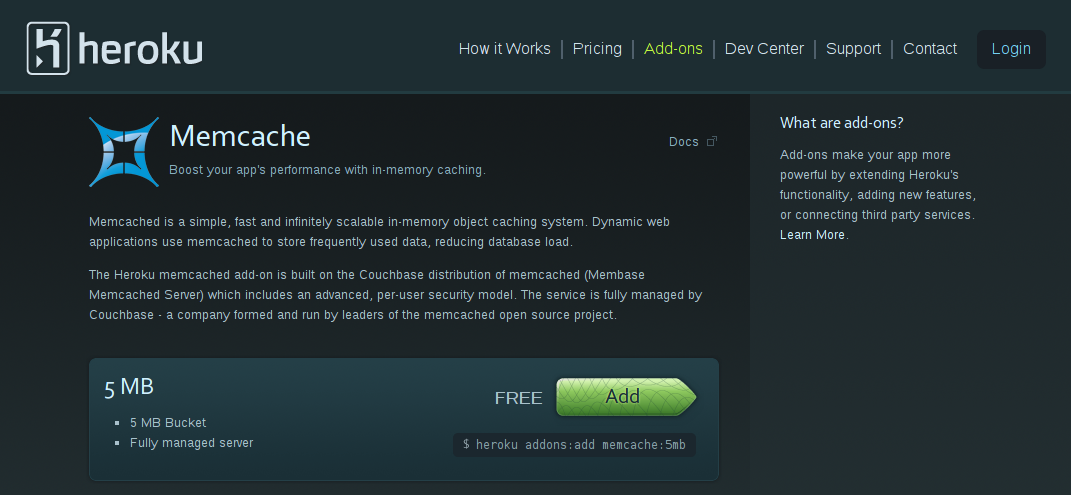
\includegraphics[scale=0.18]{figures/heroku.png}
  \end{center}
  \begin{itemize}
    \item Leading cloud service (PAAS) provider
    \item Over 1,500,000 hosted applications
    \item Couchbase Server serving over 11,800 Heroku customers
  \end{itemize}
\end{frame}
\begin{frame}[squeeze]{Who Uses Couchbase Server: Zynga}
  \begin{center}
    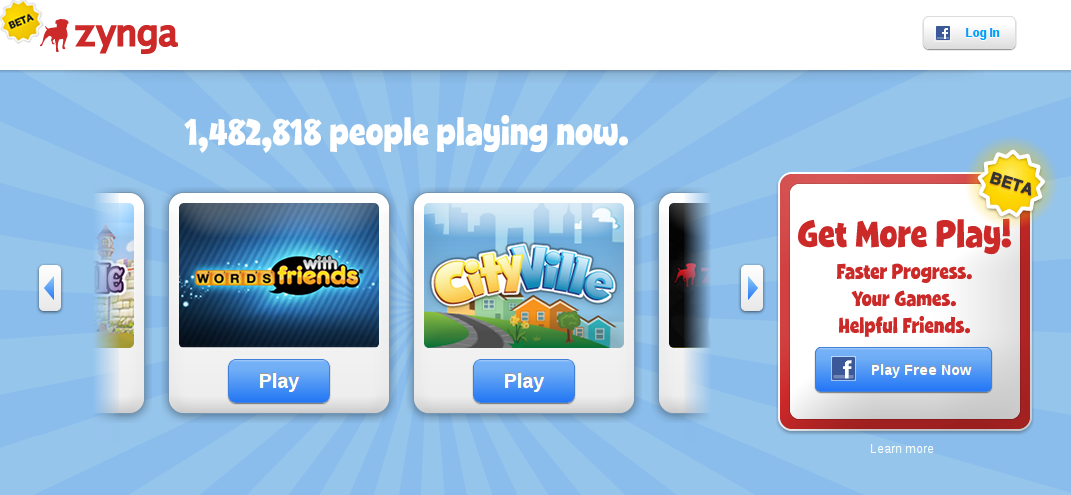
\includegraphics[scale=0.18]{figures/zynga.png}
  \end{center}
  \begin{itemize}
    \item Social game leader --- FarmVille, Mafia Wars, Empires and Allies, Café World, FishVille
    \item Over 230 million monthly users
    \item Couchbase Server is the primary database behind key Zynga properties
  \end{itemize}
\end{frame}

\section{Current Version: 1.1.2}

\begin{frame}[fragile]{Installation}
  Install stable version of \texttt{libcouchbase-dev} with dependencies using instructions at
  \href{http://www.couchbase.com/develop/c/current}{\tt http://www.couchbase.com/develop/c/\alert{current}}

  \begin{semiverbatim}
  \$ gem install couchbase
  Fetching: couchbase-1.1.2.gem (100\%)
  Building native extensions.  This could take a while...
  Successfully installed couchbase-1.1.2
  1 gems installed
  \end{semiverbatim}
\end{frame}

\begin{frame}[fragile]{Connect to the Cluster}
  Pass connection parameters explicitly
  \begin{semiverbatim}
  conn = Couchbase.\alert{connect}(:bucket => 'test')
  \end{semiverbatim}

  Use thread-local connection instance
  \begin{semiverbatim}
  Couchbase.\alert{connection_options =} {:bucket => 'test'}
  conn = Couchbase.\alert{bucket}
  \end{semiverbatim}
\end{frame}

\begin{frame}[fragile]{Simple CRUD}
  Write key or fail it it is \itshape{exists already}
  \begin{semiverbatim}
    cas = conn.\alert{add}("key", "value")
  \end{semiverbatim}
  Write key \itshape{unconditionally}
  \begin{semiverbatim}
    cas = conn.\alert{set}("key", "value")
  \end{semiverbatim}
  Write key \itshape{only if} it is \itshape{exists}
  \begin{semiverbatim}
    cas = conn.\alert{replace}("key", "value")
  \end{semiverbatim}
  \begin{semiverbatim}
    value = conn.\alert{get}("key")
  \end{semiverbatim}
\end{frame}

\begin{frame}[fragile]{Optimistic Locks}
  All mutators accepts CAS value (some kind of version or checksum of the key)

  \begin{semiverbatim}
    value, flags, \alert{cas} = conn.get("key", "value",
                                 \alert{:extended => true})
  \end{semiverbatim}

  Setting with wrong CAS value will raise \texttt{Couchbase::Error::KeyExists}

  \begin{semiverbatim}
    conn.set("key", "newvalue", \alert{:cas => 1234})
    \#=> Couchbase::Error::KeyExists: failed to store value
  \end{semiverbatim}
\end{frame}

\begin{frame}[fragile]{Expiration}
  Write key and set expiration
  \begin{semiverbatim}
    conn.set("key", "value", \alert{:ttl => 1.minute})
  \end{semiverbatim}

  Read key and set expiration
  \begin{semiverbatim}
    conn.get("key", \alert{:ttl => 1.minute})
  \end{semiverbatim}

  Only update expiration
  \begin{semiverbatim}
    conn.\alert{touch}("key", \alert{:ttl => 1.minute})
  \end{semiverbatim}
\end{frame}

\begin{frame}[fragile]{Miscellaneous}
  Multi get
  \begin{semiverbatim}
    foo, bar = conn.get("foo", "bar")
  \end{semiverbatim}

  Multi touch
  \begin{semiverbatim}
    conn.touch("foo" => 30.seconds, "bar" => 10.minutes)
  \end{semiverbatim}

  Increment/Decrement
  \begin{semiverbatim}
    conn.incr("counter")
    conn.decr("counter")
  \end{semiverbatim}
\end{frame}

\section{Next Version: 1.2.0.dp5}

\begin{frame}[fragile]{Installation}
  Install next version of \texttt{libcouchbase-dev} with dependencies using instructions at
  \href{http://www.couchbase.com/develop/c/next}{\tt{}http://www.couchbase.com/develop/c/\alert{next}}

  \begin{verbatim}
    $ gem install couchbase --pre
    Fetching: couchbase-1.2.0.dp5.gem (100%)
    Building native extensions.  This could take a while...
    Successfully installed couchbase-1.2.0.dp5
    1 gems installed
  \end{verbatim}
\end{frame}

\begin{frame}[fragile]{Map/Reduce Analysis}
  Define \alert{design document} containing single \alert{map} function
  (using admin panel or \texttt{Bucket\#save\_design\_doc}):

  \begin{verbatim}
    {
      "_id": "_design/users",
      "views": {
        "all_by_email": {
          "map": "function(doc) {
                    if (doc.type == "User")
                      emit(doc.email, null);
                  }"
        },
      }
    }
  \end{verbatim}
\end{frame}

\begin{frame}[fragile]{Executing views}
  Pick up design document:

  \begin{semiverbatim}
    ddoc = conn.design_docs["users"]
  \end{semiverbatim}

  Iterate over view results

  \begin{semiverbatim}
    ddoc.all_by_email(:include_docs => true).each do |doc|
      puts doc.key
      puts doc.doc.inspect
    end
  \end{semiverbatim}
\end{frame}

\begin{frame}[fragile]{Pessimistic Locks}
  \begin{semiverbatim}
    value = conn.get("key", \alert{:lock => 5.seconds})
  \end{semiverbatim}

  All subsequent mutators are forced to use corresponding CAS value or fail
\end{frame}

\begin{frame}[fragile]{Rack Session Storage}
  \begin{semiverbatim}
    # config.ru
    require 'rack/session/couchbase'
    use Rack::Session::Couchbase,
        :expire_after => 5.minutes,
        :couchbase => \{:bucket => "sessions"\}
  \end{semiverbatim}
\end{frame}

\begin{frame}[fragile]{Rails Session Storage}
  \begin{semiverbatim}
    # config/initializers/session\_store.rb
    require \\
      'action_dispatch/middleware/session/couchbase_store'

    {\itshape{}Name}::Application.config.session_store :couchbase_store,
                      :expire_after => 5.minutes,
                      :couchbase => \{:bucket => "sessions"\}
  \end{semiverbatim}
\end{frame}

\begin{frame}[fragile]{Rails Cache Storage}
  \begin{semiverbatim}
    # config/application.rb
    cache_options = \{
      :bucket => 'protected',
      :username => 'protected',
      :password => 'secret',
      :expires_in => 2.hours
    \}
    config.cache_store = :couchbase_store, cache_options
  \end{semiverbatim}
\end{frame}

\section{Even More :)}

\begin{frame}[fragile]{ODM (Object Document Model) for Rails}
  \href{https://github.com/couchbaselabs/ruby-couchbase-model}{\tt{}https://github.com/couchbaselabs/ruby-couchbase-model}

  \begin{semiverbatim}
    $ gem install couchbase-model
  \end{semiverbatim}

  \begin{semiverbatim}
    class Post < Couchbase::Model
      attribute :title
      attribute :body
      attribute :created\_at, :default => lambda \{ Time.now \}
      view :by\_created\_at
    end
  \end{semiverbatim}
\end{frame}

\begin{frame}[fragile]{Couchbase for EventMachine (experimental)}
  \href{https://github.com/couchbaselabs/couchbase-ruby-client-em}{\tt{}https://github.com/couchbaselabs/couchbase-ruby-client-em}

  \begin{semiverbatim}
    $ gem install em-couchbase
  \end{semiverbatim}
\end{frame}

\thanks

\sectionback
\begin{frame}
  \begin{beamercolorbox}[center]{title}
    \usebeamerfont{section title}

    Find these slides at:

    \usebeamerfont{subtitle}
    github.com/avsej/getting-started-with-couchbase-ruby
  \end{beamercolorbox}
\end{frame}
\end{document}
